\documentclass[12pt,a4paper]{tesiinfo}
\usepackage[utf8]{inputenc}
\usepackage[T1]{fontenc}
\usepackage{graphicx}
\usepackage{enumitem}
\usepackage{lmodern}
\usepackage{textcomp}
\usepackage{booktabs}
\usepackage{longtable}
%\usepackage{titlesec}
\usepackage{hyperref}
\setcounter{secnumdepth}{4}
\usepackage{rotating}
\usepackage{array}
\usepackage{makecell}
\usepackage{multirow}
\usepackage[dvipsnames,table,xcdraw]{xcolor}
\usepackage{hhline}
\usepackage[english]{babel}
\usepackage{caption}
\usepackage{amsmath}
\usepackage{tikz}
\usepackage{caption}
\usepackage{listingsutf8}

\DeclareCaptionFont{white}{\color{white}}
\DeclareCaptionFormat{listing}{%
	\parbox{\textwidth}{\colorbox{RoyalBlue}{\parbox{\textwidth}{#1#2#3}}\vskip-4pt}}
\captionsetup[lstlisting]{format=listing,labelfont=white,textfont=white}
\lstset{frame=lrb,xleftmargin=\fboxsep,xrightmargin=-\fboxsep}

\lstset{
	numbers=left,
	numberstyle=\tiny,
	numbersep=8pt,
	frame=lrb,
	xleftmargin=\fboxsep,
	xrightmargin=-\fboxsep,
	inputencoding=utf8/latin1,
	keywordstyle=\color{blue},
	commentstyle=\color{gray},
	basicstyle=\tiny\ttfamily}

\lstdefinestyle{framed}
{
	frame=blr,         
	belowcaptionskip=-1pt,
	xleftmargin=8pt,
	framexleftmargin=8pt,
	%backgroundcolor=\color{gray!10},
	framexrightmargin=5pt,
	framextopmargin=10pt,
	framexbottommargin=5pt,
	framesep=0pt,
	rulesep=0pt,
	numbersep=-4pt,
	numberstyle=\tiny\color{darkgray},
	rulecolor=\color{black}
}
\usetikzlibrary{shapes,arrows,positioning}

\graphicspath{{./Immagini/}}

\begin{document}
	
	
	\begin{titlepage}
\begin{center}
\normalsize

\begin{center}

\begin{tabular}[t]{@{} l @{} c @{} r @{}}
\parbox[c]{0.15\textwidth}{\raggedright 
\includegraphics[width=0.15\textwidth]{logo}}
&
\parbox[c]{0.7\textwidth}
{
\centering \bfseries
Università degli Studi dell'Aquila \\[-5pt]
\rule{0.6\textwidth}{1pt} \\
{\centering \small Dipartimento di Ingegneria e \\Scienze dell'Informazione e Matematica} \\
}
&
\parbox[c]{0.15\textwidth}{\raggedleft 
\includegraphics[width=0.15\textwidth]{disim}}
\end{tabular}
\end{center}

\bigskip \bigskip



\bigskip
\bigskip
\bigskip

\vfil

{\bfseries \huge
Space and Time Estimations for Well Known Algorithms: from C to RTL Implementation \\
}

{\large
\bigskip
\bigskip
\bigskip
\bigskip
{\bfseries \large Docente \\ }
\smallskip
\textbf{Prof.} \textit{Luigi Pomante} \\
\bigskip
{\bfseries \large Dottorando referente \\ }
\smallskip
\textbf{Dott.} \textit{Giacomo Valente} \\
}

{\bfseries \large
\bigskip
\bigskip


Studenti \\
}

\vfil
\vfil

\makebox[\textwidth][c]{

\begin{minipage}[t]{0.45\textwidth}
\centering
{\bfseries Angelo Damiani} \\
\bigskip
%\dotfill
\underline{\hspace{\textwidth}}
\end{minipage}

\hspace*{0.1\textwidth}

\begin{minipage}[t]{0.45\textwidth}
\centering
{\bfseries Michele Iessi} \\
\bigskip
\underline{\hspace{\textwidth}}

\end{minipage}

}

\vspace{2\baselineskip}

\makebox[\textwidth][c]{

\begin{minipage}[t]{0.45\textwidth}
\centering
{\bfseries Silvia Montecchia} \\
\bigskip
%\dotfill
\underline{\hspace{\textwidth}}
\bigskip
\bigskip
\end{minipage}



}

\vfil \vfil \vfil

\rule{\textwidth}{1pt}\\
{\scshape Anno Accademico 2017--2018}

\end{center}
\end{titlepage}
	
	\tableofcontents
	
	\chapter*{Introduction}

In the Embedded Systems context, it is important for designers to have estimations of spatial occupation and time performance for their projects in order, for example, to choose the final platform for deployment.

Our work is based on the \textit{CC4CS} project\cite{cc4cs_git}. This project aims to build a framework that is able to provide to engineers an estimation for the time their applications, written in C/C++, will take to be executed on the target platform.

If we suppose instead to use a SPP then other HLS tools are useful, such as Vivado HLS\cite{vivado_hls}. For an SPP it is fairly simple to give performance estimations, because a full hardware implementation has a worst case latency that is easier to detect with respect to a programmable processor.

We used Vivado HLS to determine those estimations for several well-known algorithms using the ZedBoard as target platform\cite{zedboard}. After the first evaluation, we improved our results through the usage of various hardware \emph{directives}. These are "rules" given to Vivado HLS in order to have better space and time performance estimations.

In chapter \ref{chapter:description}, after some experimentation to take faimiliarity with the Vivado HLS environment, we describe the context of the work and provide a list of the tested algorithms.

In chapter \ref{chapter:hardware}, we discuss about tools used in our development of the solution to the problem.

In chapter \ref{chapter:software}, we report all the parts related to software implementation of our solution to the problem.

In chapter \ref{chapter:validation}, we describe the validation activities done to demonstrate that our solution works.

In chapter \ref{chapter:conclusion}, we report conclusions of our work and future activities.

In chapter \ref{chapter:problems}, we report problems encountered during every phase of the project.
	\chapter{Description of the Work}
\label{chapter:description}
% Spieghiamo cose abbiamo fatto prima di fare il lavoro vero e proprio, comprendendo eventuali problemi incontrati
\section{Preliminary Setup and Experimentation}

Before starting our work, we followed a basic guide \cite{tutorial} for the Zynq Zedboard platform. These tutorials proved to be very useful to the team in order to grasp the basics of the platform. After setting up the environment, we built the first application, named \texttt{HelloWorld}, that simply sends its name to the UART1 interface.

% Spieghiamo come far si che il sistema si accorga della board su un sistema Linux
\subsection{Linux Configuration}

While on Windows machines the detection on the board may be automatic due to Windows Update, for a Linux system two packages are required. They are the Adept Runtime and Adept Utilities packages, that can be obtained from the Digilent website. If these two packages are not installed on the machine, then both Vivado and the SDK will not recognize the board when connected, effectively rendering impossible any kind of configuration.

% Spieghiamo come abbiamo implementato la funzionalità per misurare il tempo trascorso
\subsection{Timer Experimentation}
The first thing that we tried was a simple computation of the execution time of the \texttt{HelloWorld} application. We followed the tutorial released by AVNET modifying the \texttt{C++} code. We included the \texttt{XTime\_l.h} library. Doing this we can get the Global Timer Counter Register value in order to compute the time elapsed to print "Hello world" using the UART connection to the PC. The new code is in figure \ref{fig:helloworldtimer}.

\begin{figure}[htbp]
	\centering
	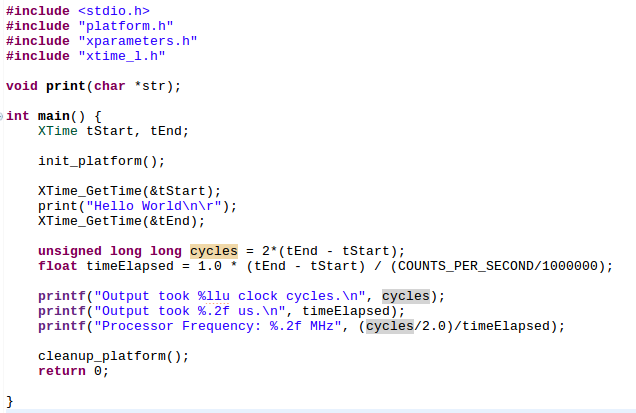
\includegraphics[width=0.85\textwidth]{timerHelloWorld}
	\caption{Time evaluation for the \texttt{HelloWorld} application}
	\label{fig:helloworldtimer}
	
	\bigskip
	\noindent
	\begin{flushleft}
		The ARM core is processing at 333 MHz, that is the configured frequency, as shown in figure \ref{fig:helloworldtimeroutput}.
	\end{flushleft}
	\bigskip
	
	\centering
	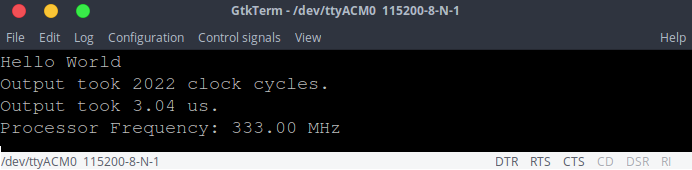
\includegraphics[width=0.85\textwidth]{GTKHelloWorldTimerOutput}
	\caption{UART output on GTKTerm (on PC)}
	\label{fig:helloworldtimeroutput}
\end{figure}

\section{Context of the Work}
% "One general scheme of your work that allows to understand where your work fits"
Our work is strictly related to the CC4CS project\cite{cc4cs_git} (acronym for \textit{Clock Cycles for C Statement}). CC4CS is the ratio between the number of clock cycles required by the processor to run an application and the number of executed C statements. A framework that helps to calculate this metric has been realized:

\[
\text{CC4CS} = \frac{\text{Number of Clock Cycles}}{\text{Executed C Statements}}
\]

This framework aims to help engineers extimate the execution time of their applications, described in C, on any platform. This would give the designer a way to work with extimates before choosing the final platform.

\subsection{Tested Algorithms}
\label{tested-algo}

The algorithms used to test the framework are the following

\begin{itemize}[noitemsep]
	\item Selection Sort
	\item Bubble Sort
	\item Merge Sort
	\item Quick Sort
	\item Insertion Sort
	\item Greatest Common Divisor
	\item Floyd-Warshall's Algorithm
	\item Bellman-Ford's Algorithm
	\item Banker's Algorithm

\end{itemize}

Time and space estimations for an initial VHDL/Verilog implementation of these algorithms are available in section \ref{sec:spacetime_estimations}. These estimations have been performed using these parameters:

\begin{itemize}[noitemsep]
	\item \textbf{Sorting Algorithms}: input array with dimension 10, with type \textbf{float} or \textbf{long}
	\item \textbf{GCD Algorithm}: testbench made using arbitrary \textbf{integer} numbers
	\item \textbf{Graph Algorithms}: input (adjacency) matrix with dimension $10\times10$
	\item \textbf{Banker's Algorithm}: testbench made using 4 processes and 3 resources

\end{itemize}
	\chapter{Hardware Implementation}
\label{chapter:hardware}
In this part we discuss about the tools used in our development of the solution to the problem stated in the introduction.

\section{Description of the Tools Used}

In this section, we will discuss about tools used in order to study the problem and develop a feasible solution.

\subsection{Vivado HLS}

Vivado High-Level Synthesis\cite{vivado_hls} is a software designed by Xilinx. It allows designers to accelerate IP creation by enabling C, C++ and System C specifications to be targeted into Xilinx devices without the need to manually create RTL. Supporting both the ISE\cite{ise} and Vivado design environments, Vivado HLS provides system and design architects alike with a faster path to IP creation by:

\begin{itemize}[noitemsep]
	\item Abstraction of algorithmic description, data type specification and interfaces
	\item Extensive library for arbitrary precision data types, video, DSP and more
	\item Directive driven architecture-aware synthesis that delivers the best possible QoR (Quality of Results)
	\item Fast time to QoR that rivals hand-coded RTL
	\item Accelerated verification using C/C++ test bench simulation, automatic VHDL or Verilog simulation and test bench generation
	\item Multi-language support
	\item Automatic use of Xilinx on-chip memories, DSP elements and floating point library
	\item Use of directives
\end{itemize}
Furthermore, Vivado HLS supports older architectures specific to ISE Design Suite and installs automatically as part of the Vivado HLx Editions. Problems and relative solutions about installation and utilization of Vivado HLS are available in section \ref{vivado_activation} and \ref{vivado_compile}.

\subsection{Generating VHDL and Verilog code using Vivado HLS}

The main feature of Vivado HLS is that it allows synthesis of C programs into Hardware Description Languages, such as VHDL or Verilog. This allows the program to be effectively ported onto an FPGA, while also providing useful informations such as space occupation and time/latency estimations.

\textit{Directives} (or \textit{Pragmas}) provide means of kernel optimization during the transition from C/C++ to VHDL/Verilog code. The goal of kernel optimization is to create processing logic that can consume all the data as soon as it arrives at the kernel interfaces. This is generally achieved by expanding the processing code to match the data path with techniques such as function pipelining, loop unrolling, array partitioning, dataflowing, etc. The attributes and pragmas described here are provided to assist your optimization effort. A complete list of appliable directives is available on the Xilinx website\cite{xilinx_directives}.

\newpage

\section{Space and Time Estimations}
\label{sec:spacetime_estimations}

Table \ref{tab:space_time_est} contains information about \textbf{Time Performance} (Estimated Period, Minimum Latency, Maximum Latency) and \textbf{Space Occupation} (DPS, FF, LUT used). We omitted the BRAM space occupation because it was 0 for all algorithms.

The \textit{CC} metric for maximum and minimum latency stands for \textit{Clock Cycles}. The red question marks for the GCD algorithm are due to the fact that it is not possible to do an \textit{a priori} estimation of these parameters, because they depend on the input. 

These estimations have been made with the directive \texttt{TRIPCOUNT}. This directive in used to set boundaries for the loops and cycles whose execution depends on program variables, and was necessary for Vivado HLS in order to give a time estimation.

\begin{table}[h]
	\centering
	\resizebox{\textwidth}{!}{%
		\begin{tabular}{l|c|c|c|r|r|r|}
			\cline{2-7}
			& \multicolumn{3}{c|}{}                                                           & \multicolumn{3}{l|}{}                                                                                    \\
			& \multicolumn{3}{c|}{\textbf{Time Performance}}                                  & \multicolumn{3}{c|}{\textbf{Space Occupation}}                                                           \\
			\multirow{-3}{*}{}                                         & \multicolumn{3}{c|}{}                                                           & \multicolumn{3}{l|}{}                                                                                    \\ \hline
			\multicolumn{1}{|c|}{\textbf{Algorithm}}                   & \textit{Estimated Period (\textit{ns})} & \textit{Min. Latency (\textit{CC})}    & \textit{Max. Latency (\textit{CC})}    & \multicolumn{1}{c|}{\textit{DSP}} & \multicolumn{1}{c|}{\textit{FF}} & \multicolumn{1}{c|}{\textit{LUT}} \\ \hline
			\multicolumn{1}{|l|}{Selection Sort}                       & 6.79                      & 73                       & 361                      & 0                                 & 229                              & 436                               \\
			\rowcolor[HTML]{DDDDDD} 
			\multicolumn{1}{|l|}{\cellcolor[HTML]{DDDDDD}Bubble Sort}  & 7.64                      & 3                        & 223                      & 0                                 & 551                              & 276                               \\
			\multicolumn{1}{|l|}{Merge Sort}                           & 7.59                      & 61                       & 1270                     & 0                                 & 3061                             & 1351                              \\
			\rowcolor[HTML]{DDDDDD} 
			\multicolumn{1}{|l|}{\cellcolor[HTML]{DDDDDD}Quick Sort}   & 7.53                      & 2                        & 4911                     & 0                                 & 2373                             & 902                               \\
			\multicolumn{1}{|l|}{Insertion Sort}                       & 6.79                      & 28                       & 424                      & 0                                 & 260                              & 409                               \\
			\rowcolor[HTML]{DDDDDD} 
			\multicolumn{1}{|l|}{\cellcolor[HTML]{DDDDDD}GCD}          & 7.34                      & {\color[HTML]{FE0000} ?} & {\color[HTML]{FE0000} ?} & 2                                 & 550                              & 1263                              \\
			\multicolumn{1}{|l|}{Floyd-Warshall}                       & 6.52                      & 3221                     & 3221                     & 0                                 & 391                              & 248                               \\
			\rowcolor[HTML]{DDDDDD} 
			\multicolumn{1}{|l|}{\cellcolor[HTML]{DDDDDD}Bellman-Ford} & 8.73                      & 453                      & 8453                     & 2                                 & 2196                             & 2542                              \\
			\multicolumn{1}{|l|}{Banker's Algorithm}                   & 8.44                      & 8                        & 69                       & 0                                 & 877                              & 370                               \\ \hline
		\end{tabular}%
	}
	\caption{Time and Space estimations for the algorithms with no directive (except TRIPCOUNT)}
	\label{tab:space_time_est}
\end{table}


	\chapter{Software Implementation}
\label{chapter:software}
In this chapter we discuss about our work in splitting the \texttt{.c} files from the CC4CS Github repository\cite{cc4cs_git} to \texttt{.c} and \texttt{.h} files that can be used with Vivado HLS. They have been pushed into a repository\cite{repo_our_files}.

After this, we describe our workflow in implementing and testing the correctness of our software and hardware implementations of the described algorithms.

\section{General Workflow}

The first thing we did was to split the original C file into 3 separate files:

\begin{itemize}[noitemsep]
	\item \textbf{Algorithm \texttt{.c} and \texttt{.h} files}
	\begin{itemize}[noitemsep]
		\item \texttt{.c} file: this file contains the code for the chosen algorithm
		\item \texttt{.h} file: this file contains the definitions for important constants (\textit{e.g.}: input dimension), data types, iterator types and functions of the chosen algorithm
	\end{itemize}
	\item \textbf{Algorithm testbench file}: this file generates input data and verifies that both the software and VHDL simulation (\textbf{Co-Simulation}) produce the same results
\end{itemize}


The general workflow diagram is shown in figure \ref{figure:translation}.
\newpage
\begin{figure}[ht]
	\begin{center}
		\begin{tikzpicture}[auto, node distance=1.2cm,>=latex']

		
		\node[] (c-original) {
			
\includegraphics[scale=.3]{c_redefined}};
		\node[below=0.1cm of c-original] {C original file};
		\node[below right = 3cm of c-original] (ch-translated) {
			
\includegraphics[scale=.2]{c+h_redefined}};
		\node[below=0.1cm of ch-translated] (ch-tooltip) {C and Header files};
		\node[below left = 3cm of c-original] (c-testbench) {
			
\includegraphics[scale=.3]{c_redefined}};
		\node[below=0.1cm of c-testbench] (testbench-tooltip) {C testbench file};
		\node[below=3cm of ch-translated] (vhdl) {
			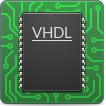
\includegraphics[scale=.8]{vhdl}};
		\node[below=0.1cm of vhdl] (vhdl-tooltip) {VHDL files};
		\node[left=1cm of c-testbench] (resultMid) {};		
		\node[above=0.1cm of resultMid] (resultPass) {
			\textit{\color{ForestGreen}{Passed}}};
		\node[below=0.1cm of resultMid] (resultNot) {
			\textit{\color{red}{Not Passed}}};
		
		\draw [->,>=latex] (c-original) -| (ch-translated);
		\draw [->,>=latex] (c-original) -| (c-testbench);
		\draw [->,>=latex] (ch-tooltip) -- node[] {Synthesis} (vhdl);
		\draw [->,>=latex] (vhdl) -| node[above right] {Co-Simulation} (testbench-tooltip);
 		\draw [->,>=latex] (ch-translated) -- node[above] {Co-Simulation} (c-testbench);
 		\draw [->,>=latex] (c-testbench) -- (resultMid);
		\end{tikzpicture}
		
	\end{center}
	\caption{Workflow}
	\label{figure:translation}
	
\end{figure}

\newpage
\section{Algorithm File Splitting Example}

Here we describe the process of splitting a .c file from the original repository to a .c and .h file. As we said earlier, this process allows to customize data input types and sizes. We did this to give other developers the possibility to evaluate the same algorithms by using different input formats.

As an example, we show this process for the MergeSort algorithm shown in Listing \ref{lst:mergesort_original}.

\begin{lstlisting}[label=lst:mergesort_original,caption=Original Mergesort Code,language=C,tabsize=4]
#include <stdint.h>
#include <values.h>
#include <8051.h>

typedef long TARGET_TYPE;
typedef int8_t TARGET_INDEX;
void prototype(long size, long a[size]);
TARGET_INDEX h = 0;

void resetValues() {
	P0 = 0;
	P1 = 0;
	P2 = 0;
	P3 = 0;
}

void merge(TARGET_INDEX i1, TARGET_TYPE f1, TARGET_TYPE f2) {
	TARGET_TYPE x[size];
	TARGET_INDEX i2 = f1 + 1;
	TARGET_INDEX i = 0;
	TARGET_TYPE start = i1;	
	
	while(i1 <= f1 && i2 <= f2) {
		if(a[i1] <= a[i2])
		x[i++] = a[i1++];
		else
		x[i++] = a[i2++];
	}
	if(i1 <= f1) {
		for(h = i1; h <= f1; h++) 
			x[i++] = a[h];
	}
	else {
		for(h = i2; h <= f2; h++)
			x[i++] = a[h];
	}
	for(h = start, i = 0;h <= f2; h++)
		a[h] = x[i++];
}

TARGET_TYPE min(TARGET_TYPE c, TARGET_TYPE b) {
	return c < b ? c : b;
}

void mergesort() {
	TARGET_TYPE m = 0;
	TARGET_TYPE x = 0;
	
	for(m = 1; m <= size-1; m *= 2) {
		for(x = 0; x < size-1; x += (2*m)) {
			merge(x, x+m-1, min(x + 2*m - 1, size-1));
		}
	}
}

void main() {
	mergesort();
	resetValues();
}
\end{lstlisting}


It is worth noting that this code has been partially refactored to better fit in this report. Also, the original code had \texttt{for} cycles that were spanned on 3 lines. This was made in this way to let the profiler (\texttt{gcov}) correctly counting C statements in the original \textit{CC4CS} project. Therefore, we only used one line for the sake of visualization.

\subsection{Removed and Moved Code}

The first main modification done on the code was the removal of the \texttt{resetValues()} method. The duty of this method was to give a stop condition when the algorithm was run onto an 8051 Microcontroller. Other parts were removed for the same reason (line \texttt{3} and \texttt{52}).

The second modification on the code was the creation a header file and the moving of parts of the code within it. This allows for great customizability and code reuse, as the .c file is independent from data types. More specifically, the variables moved inside the header file were \texttt{TARGET\_TYPE} and \texttt{TARGET\_INDEX}. A \texttt{define} named \texttt{SIZE} was also added to let the developer choose the size of the input.

The code shown in Listings \ref{lst:mergesort_header} and \ref{lst:mergesort_c} represent the final \texttt{.h} and \texttt{.c} files.

\bigskip

\begin{lstlisting}[label=lst:mergesort_header,caption=Mergesort Header File,language=C,tabsize=4]
#ifndef __MERGESORT_H__
#define __MERGESORT_H__

#include <stdint.h>

#define SIZE 10

typedef long TARGET_TYPE;
typedef long TARGET_INDEX;

void mergesort(long arr[SIZE]);

#endif
\end{lstlisting}

\newpage

\begin{lstlisting}[label=lst:mergesort_c,caption=Mergesort C File,language=C,tabsize=4]
#include "mergesort.h"

int8_t h = 0;

void merge(TARGET_INDEX i1, TARGET_INDEX f1, TARGET_INDEX f2, TARGET_TYPE arr[SIZE]) {
	TARGET_TYPE x[SIZE];
	TARGET_INDEX i2 = f1 + 1;
	TARGET_INDEX i = 0;
	TARGET_TYPE start = i1;
	
	MERGE_WHILE:
	while(i1 <= f1 && i2 <= f2) {
		if(arr[i1] <= arr[i2])
		x[i++] = arr[i1++];
		else
		x[i++] = arr[i2++];
	}	
	if(i1 <= f1) {
	MERGE_FOR1:
	for(h = i1; h <= f1; h++)
		x[i++] = arr[h];
	}
	else {
	MERGE_FOR2:
	for(h = i2;	h <= f2; h++)
		x[i++] = arr[h];
	}
	MERGE_FOR3:
	for(h = start, i = 0; h <= f2; h++)
	arr[h] = x[i++];
}

TARGET_TYPE min(TARGET_TYPE c, TARGET_TYPE b) {
	return c < b ? c : b;
}

void mergesort(TARGET_TYPE arr[SIZE]) {
	TARGET_INDEX m = 0;
	TARGET_INDEX x = 0;
	FOR1:
	for(m = 1; m <= SIZE-1; m *= 2) {
		FOR2:
		for(x = 0; x < SIZE-1; x += (2*m)) {
			merge(x, x+m-1, min(x + 2*m - 1, SIZE-1), arr);
		}
	}
}
\end{lstlisting}

% scrivere a che servono i label













	\chapter{Validation}
\label{chapter:validation}
With respect to Table \ref{tab:space_time_est}, the team tried to improve overall space occupation and time performances by applying \emph{directives} (or \emph{pragmas}) in each project. A summary description of several directives is in section \ref{sec:directives}. Finally, it is possible to see a recap of this final step in Table \ref{tab:space_time_dir}.

\section{Directives}
\label{sec:directives}

In this section we summarize the directives used in various step of Vivado HLS usage. A complete and detailed list of all directives has been written on the Xilinx website \cite{xilinx_directives}.

\subsection{\texttt{loop\_tripcount}}

The \texttt{\textbf{TRIPCOUNT}} pragma can be applied to a loop to manually specify the total number of iterations performed by a loop. It is important to know that the \texttt{\textbf{TRIPCOUNT}} pragma is for analysis only, and does not impact the results of synthesis.

Vivado HLS reports the total latency of each loop, which is the number of clock cycles to execute all iterations of the loop. The loop latency is therefore a function of the number of loop iterations, or tripcount.

The \texttt{\textbf{TRIPCOUNT}} can be a constant value. It may depend on the value of variables used in the loop expression (for example, $x<y$), or depend on control statements used inside the loop. In some cases Vivado HLS cannot determine the tripcount, and the latency is unknown. This includes cases in which the variables used to determine the tripcount are:
\begin{itemize} [noitemsep]
	\item Input arguments
	\item Variables calculated by dynamic operations
\end{itemize}

In cases where the loop latency is unknown or cannot be calculate, the \texttt{\textbf{TRIPCOUNT}} pragma lets you specify minimum and maximum iterations for a loop. This lets the tool analyze how the loop latency contributes to the total design latency in the reports, and helps you determine appropriate optimizations for the design.

In our implementation, we used this directive and gave it a value based on the minimum, average and worst case, depending on the loop variables.

\subsection{\texttt{pipeline}}

The \texttt{\textbf{PIPELINE}} pragma reduces the initiation interval for a function or loop by allowing the concurrent execution of operations. Pipelining a loop allows the operations of the loop to be implemented in a concurrent manner.

A pipelined function or loop can process new inputs every N clock cycles, where N is the initiation interval (\textit{II}) of the loop or function. The default initiation interval for the \texttt{\textbf{PIPELINE}} pragma is 1, which processes a new input every clock cycle. It is also possible to specify the initiation interval through the use of the II option for the pragma.

If Vivado HLS cannot create a design with the specified II, it:
\begin{itemize}[noitemsep]
	\item Issues a warning
	\item Creates a design with the lowest possible II
\end{itemize}

It is possible to analyze this design with the warning message to determine what steps must be taken to create a design that satisfies the required initiation interval.

\newpage
\subsection{\texttt{array\_partition}}

The \texttt{\textbf{ARRAY\_PARTITION}} pragma partitions an array into smaller arrays or individual elements. This partitioning:
\begin{itemize}[noitemsep]
	\item Results in RTL with multiple small memories or multiple registers instead of one large memory
	\item Effectively increases the amount of read and write ports for the storage
	\item Potentially improves the throughput of the design
	\item Requires more memory instances or registers
\end{itemize}

The \texttt{\textbf{ARRAY\_PARTITION}} directive has been extensively used in ordering algorithms, due to the fact that input values were arrays.

\subsection{\texttt{\textbf{unroll}}}

The \texttt{\textbf{UNROLL}} pragma unroll loops to create multiple independent operations rather than a single collection of operations. It transforms loops by creating multiples copies of the loop body in the RTL design, which allows some or all loop iterations to occur in parallel.

Loops in the C/C++ functions are kept rolled by default. When loops are rolled, synthesis creates the logic for one iteration of the loop, and the RTL design executes this logic for each iteration of the loop in sequence. A loop is executed for the number of iterations specified by the loop induction variable. The number of iterations might also be impacted by logic inside the loop body (for example, break conditions or modifications to a loop exit variable). Using the \texttt{\textbf{UNROLL}} pragma you can unroll loops to increase data access and throughput.

The \texttt{\textbf{UNROLL}} pragma allows the loop to be fully or partially unrolled. Fully unrolling the loop creates a copy of the loop body in the RTL for each loop iteration, so the entire loop can be run concurrently. Partially unrolling a loop lets you specify a factor \textit{N}, to create \textit{N} copies of the loop body and reduce the loop iterations accordingly. To unroll a loop completely, the loop bounds must be known at compile time. This is not required for partial unrolling.

Partial loop unrolling does not require \textit{N} to be an integer factor of the maximum loop iteration count. Vivado HLS adds an exit check to ensure that partially unrolled loops are functionally identical to the original loop.

When pragmas like \texttt{\textbf{DATA\_PACK}}, \texttt{\textbf{ARRAY\_PARTITION}}, or \texttt{\textbf{ARRAY\_RESHAPE}} are used, in order to let more data be accessed in a single clock cycle, Vivado HLS automatically unrolls any loops consuming this data (if doing so improves the throughput). The loop can be fully or partially unrolled to create enough hardware to consume the additional data in a single clock cycle. This feature is controlled using the \texttt{config\_unroll} command.

\subsection{\texttt{inline}}

The \texttt{\textbf{INLINE}} pragma removes a function as a separate entity in the hierarchy. After inlining, the function is dissolved into the calling function and no longer appears as a separate level of hierarchy in the RTL. In some cases, inlining a function allows operations within the function to be shared and optimized more effectively with surrounding operations. An inlined function cannot be shared. This can increase area required for implementing the RTL.

The \texttt{\textbf{INLINE}} pragma applies differently to the scope it is defined in depending on how it is specified:
\begin{itemize}
\item \texttt{INLINE}: Without arguments, the pragma means that the function it is specified in should be inlined upward into any calling functions or regions.
\item \texttt{INLINE OFF}: Specifies that the function it is specified in should NOT be inlined upward into any calling functions or regions. This disables the inline of a specific function that may be automatically inlined, or inlined as part of a region or recursion.
\item \texttt{INLINE REGION}: This applies the pragma to the region or the body of the function it is assigned in. It applies downward, inlining the contents of the region or function, but not inlining recursively through the hierarchy.
\item \texttt{INLINE RECURSIVE}: This applies the pragma to the region or the body of the function it is assigned in. It applies downward, recursively inlining the contents of the region or function.
\end{itemize}
By default, inlining is only performed on the next level of function hierarchy, not sub-functions. However, the recursive option lets you specify inlining through levels of the hierarchy.

In our case, we used the \texttt{INLINE OFF} specification of this directive for the Floyd-Warshall's algorithm.

\section{Final Results}

The application of different directives for the algorithms produced the results in Table \ref{tab:space_time_dir}.

\begin{table}[h]
	\centering
	\resizebox{\textwidth}{!}{%
		\begin{tabular}{l|l|c|c|c|r|r|r|}
			\cline{3-8}
			\multicolumn{2}{l|}{}                                                                                                                        & \multicolumn{3}{c|}{}                                                             & \multicolumn{3}{l|}{}                                                                                    \\
			\multicolumn{2}{l|}{}                                                                                                                        & \multicolumn{3}{c|}{\textbf{Time Performance}}                                    & \multicolumn{3}{c|}{\textbf{Space Occupation}}                                                           \\
			\multicolumn{2}{l|}{\multirow{-3}{*}{}}                                                                                                      & \multicolumn{3}{c|}{}                                                             & \multicolumn{3}{l|}{}                                                                                    \\ \hline
			\multicolumn{1}{|c|}{\textbf{Algorithm}}                   & \multicolumn{1}{c|}{\textbf{Directives}}                                        & \textit{Estimated Period (ns)}   & \textit{Min. Latency (CC)}    & \textit{Max. Latency (CC)}    & \multicolumn{1}{c|}{\textit{DSP}} & \multicolumn{1}{c|}{\textit{FF}} & \multicolumn{1}{c|}{\textit{LUT}} \\ \hline
			\multicolumn{1}{|l|}{Selection Sort}                       & ARRAY\_PARTITION                                                                & 8.73                        & 127                      & 271                      & 0                                 & 2353                             & 2120                              \\
			\rowcolor[HTML]{DDDDDD} 
			\multicolumn{1}{|l|}{\cellcolor[HTML]{DDDDDD}Bubble Sort}  & TRIPCOUNT                                                                       & 7.64                        & 3                        & 223                      & 0                                 & 551                              & 276                               \\
			\multicolumn{1}{|l|}{Merge Sort}                           & \begin{tabular}[c]{@{}l@{}}TRIPCOUNT\\ ARRAY\_PARTITION\\ PIPELINE\end{tabular} & 7.59                        & 57                       & 909                      & 0                                 & 3802                             & 1770                              \\
			\rowcolor[HTML]{DDDDDD} 
			\multicolumn{1}{|l|}{\cellcolor[HTML]{DDDDDD}Quick Sort}   & \begin{tabular}[c]{@{}l@{}}TRIPCOUNT\\ ARRAY\_PARTITION\\ PIPELINE\end{tabular} & 8.68                        & 1                        & 2581                     & 0                                 & 3914                             & 1606                              \\
			\multicolumn{1}{|l|}{Insertion Sort}                       & \begin{tabular}[c]{@{}l@{}}TRIPCOUNT\\ ARRAY\_PARTITION\end{tabular}            & 8.37                        & 28                       & 325                      & 0                                 & 912                              & 1094                              \\
			\rowcolor[HTML]{DDDDDD} 
			\multicolumn{1}{|l|}{\cellcolor[HTML]{DDDDDD}GCD}          & -                                                                               & 7.34                        & {\color[HTML]{FE0000} ?} & {\color[HTML]{FE0000} ?} & 2                                 & 550                              & 1263                              \\
			\multicolumn{1}{|l|}{Floyd-Warshall}                       & \begin{tabular}[c]{@{}l@{}}INLINE (off)\\ PIPELINE\end{tabular}                 & {\color[HTML]{FE0000} 9.42} & 2003                     & 2003                     & 0                                 & 423                              & 370                               \\
			\rowcolor[HTML]{DDDDDD} 
			\multicolumn{1}{|l|}{\cellcolor[HTML]{DDDDDD}Bellman-Ford} & \begin{tabular}[c]{@{}l@{}}TRIPCOUNT\\ UNROLL\end{tabular}                      & 8.73                        & 446                      & 8446                     & 2                                 & 2178                             & 2620                              \\
			\multicolumn{1}{|l|}{Banker's Algorithm}                   & \begin{tabular}[c]{@{}l@{}}UNROLL\\ PIPELINE\end{tabular}                       & {\color[HTML]{FE0000} 9.85} & 6                        & 37                       & 0                                 & 1473                             & 997                               \\ \hline
		\end{tabular}%
	}
	\caption{Time and Space estimations for the algorithms with relative directives applied}
	\label{tab:space_time_dir}
\end{table}

Values in red are due to different reasons:

\begin{itemize}
	\item For \texttt{GCD}, it is impossible to predict minimum and maximum latency (in clock cycles) because it depends on the input
	\item For \texttt{Floyd-Warshall} and \texttt{Banker's Algorithm}, the Estimated Period exceeds the maximum value for the board, that is:
	\begin{align*}
	\text{Clock} - \text{Uncertainty} = 10 \text{ ns} - 1.25 \text{ ns} = 8.75 \text{ ns}
	\end{align*}
\end{itemize}







	\chapter{Conclusion and Future Activities}
\label{chapter:conclusion}

In this document we showed that using directives it is possible to improve performance estimations for the specified algorithms, under the assumption that input type and dimension are known. This may be used by designers to have estimations of spatial occupation and time performance for their projects in order, for example, to choose the final platform for deployment.

\section{Future Activities}

Future activities for this project could be:

\begin{itemize}[noitemsep]
	\item Using different input dimensions, since our estimations were only for few input dimensions (described in section \ref{tested-algo}), one for each algorithm
	\item Using different input/output data types, since our implementation let the developer choose which to use, but for simplicity purposes we used only few of them (described in section \ref{tested-algo})
	\item Test more directives
	\item Test other algorithms
\end{itemize}

\newpage

\subsection*{Considerations About Integration with CC4CS}

Our team thought about developing scripts (in Python, Perl or sh) to automate the process of creating new input data of different dimension and type, in order to test time performance for different kinds of input. 

It is worth noticing that this process would be only useful in the co-simulation phase, because the phase of C Synthesis only gives information about space and time performance for the algorithm, considering only the \textbf{input data type} and not the input \textit{per se}.

So our team believes that such a result would be possible to achieve, given the following constraints:

\begin{itemize}
	\item For the phase of \textbf{C Synthesis}:
	\begin{itemize}
		\item The script should edit the \texttt{.h} file for each algorithm, in order to modify input dimension and data type
		\item A series of \emph{API} should be available for Vivado HLS, or at least some access points to the program, in order to start automatically the process of Synthesis and from which retrieve the results (such as those visible in table \ref{tab:space_time_dir})
		\item Enough time for the execution of multiple C Synthesis phases. On a medium-high end machine, this phase took about 7-8 seconds to execute
	\end{itemize}
	\item For the phase of \textbf{Co-Simulation}:
	\begin{itemize}
		\item All previous points
		\item It would be necessary to edit all testbench files to let them accept optional parameters (input array/matrices) from console
		\item Enough time for the execution of multiple Co-Simulation phases. On a medium-high end machine, this phase took about 15-20 seconds for input
	\end{itemize}
\end{itemize}

In conclusion, this process should be doable given the presence of a Vivado HLS access point from console/API. Moreover, if such access points existed, it would be also possible to change the target platform \textit{on demand}, and completely integrate Vivado HLS with the \textit{CC4CS} framework.
	\chapter{Problems Encountered}
\label{chapter:problems}
In this chapter we will discuss about problems encountered during every phase of the project.

\section{Vivado License Activation on Ubuntu}
\label{vivado_activation}
License activation for Vivado requires the MAC address of the main network peripheral of the machine. The License Manager looks for any peripheral named \textit{eth*}, where * can be any number. Due to the fact that many laptops and notebooks don't have peripherals named in such way, the Host ID of the machine is listed as all zeros. Thus, it is necessary to manually rename them in order to be found by the License Manager, under the \textit{Host Information} section.

The procedure is as follows: first it is necessary to issue a \texttt{ifconfig} command to the terminal, in order to see the MAC address of the network wireless adapter of the laptop (for example aa:bb:cc:dd:ee:ff). After this, another command must be issued:

\texttt{sudo nano /etc/udev/rules.d/10-network.rules}

This will create a file named \textit{10-network.rules} inside the \texttt{udev} folder. In this file it is necessary to write a single line:

\begin{scriptsize}
\texttt{SUBSYSTEM=="net", ACTION=="add", ATTR{address}=="aa:bb:cc:dd:ee:ff", NAME="eth0"}
\end{scriptsize}
\\*
This will rename the network adapter to \textit{eth0}, but any number will do. After this, rebooting the machine and executing again the License Manager will correctly show the Host ID under the Host Informations section.

\section{Compile Errors for Vivado HLS Labs on Ubuntu}
\label{vivado_compile}
There can be issues when compiling lab files in the Vivado HLS tutorial. To solve them, the procedure is to install the packet \texttt{libc6-dev-i386} (when on a 64 bit machine). After that, two more commands are required in order to compile successfully:

\texttt{LIBRARY\_PATH=/usr/lib/x86\_64-linux-gnu:\$LIBRARY\_PATH}

\texttt{export LIBRARY\_PATH}

Now there are no more problems when issueing the \texttt{make} command.
	
	\listoffigures
	
	\bibliografia{main}
	
\end{document}